% Graphic for TeX using PGF
% Title: C:\Documents and Settings\antoine.deroquemaure\Mes documents\stage\rapport\images\2-activite\bdNouvelle.dia
% Creator: Dia v0.97.2
% CreationDate: Thu Jun 14 10:37:26 2012
% For: antoine.deroquemaure
% \usepackage{tikz}
% The following commands are not supported in PSTricks at present
% We define them conditionally, so when they are implemented,
% this pgf file will use them.
\ifx\du\undefined
  \newlength{\du}
\fi
\setlength{\du}{15\unitlength}
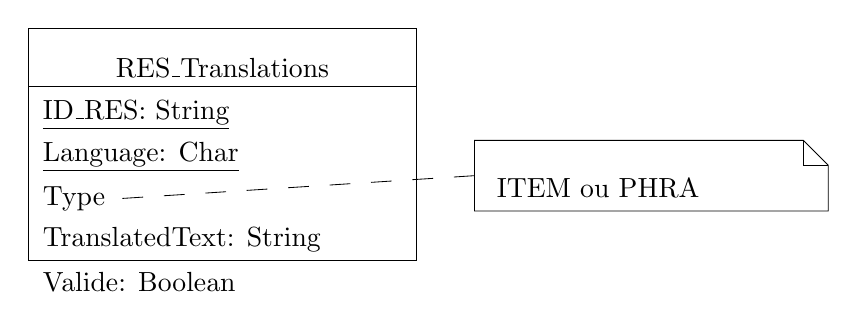
\begin{tikzpicture}
\pgftransformxscale{1.000000}
\pgftransformyscale{-1.000000}
\definecolor{dialinecolor}{rgb}{0.000000, 0.000000, 0.000000}
\pgfsetstrokecolor{dialinecolor}
\definecolor{dialinecolor}{rgb}{1.000000, 1.000000, 1.000000}
\pgfsetfillcolor{dialinecolor}
\pgfsetlinewidth{0.030000\du}
\pgfsetdash{}{0pt}
\definecolor{dialinecolor}{rgb}{1.000000, 1.000000, 1.000000}
\pgfsetfillcolor{dialinecolor}
\fill (17.850000\du,14.900000\du)--(17.850000\du,16.300000\du)--(27.205000\du,16.300000\du)--(27.205000\du,14.900000\du)--cycle;
\definecolor{dialinecolor}{rgb}{0.000000, 0.000000, 0.000000}
\pgfsetstrokecolor{dialinecolor}
\draw (17.850000\du,14.900000\du)--(17.850000\du,16.300000\du)--(27.205000\du,16.300000\du)--(27.205000\du,14.900000\du)--cycle;
% setfont left to latex
\definecolor{dialinecolor}{rgb}{0.000000, 0.000000, 0.000000}
\pgfsetstrokecolor{dialinecolor}
\node at (22.527500\du,15.850000\du){RES\_Translations};
\definecolor{dialinecolor}{rgb}{1.000000, 1.000000, 1.000000}
\pgfsetfillcolor{dialinecolor}
\fill (17.850000\du,16.300000\du)--(17.850000\du,20.500000\du)--(27.205000\du,20.500000\du)--(27.205000\du,16.300000\du)--cycle;
\definecolor{dialinecolor}{rgb}{0.000000, 0.000000, 0.000000}
\pgfsetstrokecolor{dialinecolor}
\draw (17.850000\du,16.300000\du)--(17.850000\du,20.500000\du)--(27.205000\du,20.500000\du)--(27.205000\du,16.300000\du)--cycle;
% setfont left to latex
\definecolor{dialinecolor}{rgb}{0.000000, 0.000000, 0.000000}
\pgfsetstrokecolor{dialinecolor}
\node[anchor=west] at (17.965000\du,17.00000\du){\underline{ID\_RES: String}};
% setfont left to latex
\definecolor{dialinecolor}{rgb}{0.000000, 0.000000, 0.000000}
\pgfsetstrokecolor{dialinecolor}
\node[anchor=west] at (17.965000\du,18.000000\du){\underline{Language: Char}};
% setfont left to latex
\definecolor{dialinecolor}{rgb}{0.000000, 0.000000, 0.000000}
\pgfsetstrokecolor{dialinecolor}
\node[anchor=west] at (17.965000\du,19.00000\du){Type};
% setfont left to latex
\definecolor{dialinecolor}{rgb}{0.000000, 0.000000, 0.000000}
\pgfsetstrokecolor{dialinecolor}
\node[anchor=west] at (17.965000\du,20.00000\du){TranslatedText: String};
% setfont left to latex
\definecolor{dialinecolor}{rgb}{0.000000, 0.000000, 0.000000}
\pgfsetstrokecolor{dialinecolor}
\node[anchor=west] at (17.965000\du,21.00000\du){Valide: Boolean};
\pgfsetlinewidth{0.020000\du}
\pgfsetdash{}{0pt}
\definecolor{dialinecolor}{rgb}{1.000000, 1.000000, 1.000000}
\pgfsetfillcolor{dialinecolor}
\fill (28.600000\du,17.600000\du)--(36.520000\du,17.600000\du)--(37.120000\du,18.200000\du)--(37.120000\du,19.300000\du)--(28.600000\du,19.300000\du)--cycle;
\definecolor{dialinecolor}{rgb}{0.000000, 0.000000, 0.000000}
\pgfsetstrokecolor{dialinecolor}
\draw (28.600000\du,17.600000\du)--(36.520000\du,17.600000\du)--(37.120000\du,18.200000\du)--(37.120000\du,19.300000\du)--(28.600000\du,19.300000\du)--cycle;
\pgfsetlinewidth{0.010000\du}
\definecolor{dialinecolor}{rgb}{0.000000, 0.000000, 0.000000}
\pgfsetstrokecolor{dialinecolor}
\draw (36.520000\du,17.600000\du)--(36.520000\du,18.200000\du)--(37.120000\du,18.200000\du);
% setfont left to latex
\definecolor{dialinecolor}{rgb}{0.000000, 0.000000, 0.000000}
\pgfsetstrokecolor{dialinecolor}
\node[anchor=west] at (28.910000\du,18.742500\du){ITEM ou PHRA};
\pgfsetlinewidth{0.020000\du}
\pgfsetdash{{1.000000\du}{1.000000\du}}{0\du}
\pgfsetdash{{0.500000\du}{0.500000\du}}{0\du}
\pgfsetbuttcap
{
\definecolor{dialinecolor}{rgb}{0.000000, 0.000000, 0.000000}
\pgfsetfillcolor{dialinecolor}
% was here!!!
\definecolor{dialinecolor}{rgb}{0.000000, 0.000000, 0.000000}
\pgfsetstrokecolor{dialinecolor}
\draw (28.600000\du,18.450000\du)--(19.972315\du,19.007748\du);
}
\end{tikzpicture}
